%\documentclass[notes,10pt,aspectratio=169]{beamer}

%\documentclass[notes, 10pt,aspectratio=169]{beamer}
\documentclass[10pt,aspectratio=169]{beamer}


% Add this line to your preamble
\setbeameroption{show notes on second screen=right}

%\usetheme{Singapore} %Boadilla, Madrid, default, etc. 
\usetheme[progressbar=frametitle]{metropolis}
\usecolortheme{rose} %beaver, dolphin, crane, 


%\setbeamersize{text margin left=4mm, text margin right=4mm}


\usecolortheme{default}

\usepackage[utf8]{inputenc}
\usepackage[T1]{fontenc}
\usepackage{lmodern}
\usepackage{xcolor}
\usepackage{tikz}
\usetikzlibrary{shapes.geometric, arrows, positioning}

\tikzstyle{block} = [rectangle, draw, text width=4cm, align=center, rounded corners, minimum height=1cm]
\tikzstyle{decision} = [rectangle, draw, text width=5cm, align=center, fill=blue!10, rounded corners, minimum height=1cm]
\tikzstyle{terminal} = [rectangle, draw, text width=4.5cm, align=center, fill=yellow!30, rounded corners, minimum height=1cm]
\tikzstyle{end} = [rectangle, draw, text width=5cm, align=center, fill=green!30, rounded corners, minimum height=1cm]
\tikzstyle{arrow} = [->, thick]



\usepackage{adjustbox}
%2. change the bullets 
\setbeamertemplate{itemize item}[triangle] %circle, square,... 


% 1. Define custom colors and set colors 
%\definecolor{myblue}{HTML}{003366}
\definecolor{accent}{RGB}{78,205,196}

%\setbeamercolor{title}{fg=white,bg=myblue}
\setbeamercolor{frametitle}{fg=black,bg=white}
%\setbeamercolor{normal text}{fg=mygray}
\setbeamercolor{block title}{fg=black,bg=blue}
%\setbeamercolor{block body}{fg=black,bg=white}

\setbeamercolor{item}{fg= orange!80} % Change bullet color
\setbeamercolor{button}{bg=orange, fg=white}





% 3. BibLaTeX settings
\usepackage[
  backend=biber,
  style=apa,
  citestyle=authoryear
]{biblatex}
\addbibresource{references.bib}

\title{Aftermarkets: Evidence from a Centralized Annuities System}
%\subtitle{A Mini Literature Overview}

\author{%
 Lucas Condeza
\inst{1} \and
   %\and
%  Coauthor Three\inst{3}
}
\institute{
  \inst{1} Yale University \\
}

\date{\today}

\begin{document}

\begin{frame}
  \titlepage
\end{frame}


 
\begin{frame}{Research question}
    
\begin{itemize}
    
    \item What is the impact of Aftermarkets? \textcolor{red}{[Is the question interesting? ]}

    \begin{itemize}

    \item \textbf{What are \textit{Aftermarkets}?} Sellers bid prices then buyers either buy at bidded price or bargain to improve the offer of sellers. The bargaining is costly. \textcolor{red}{[Is aftermarket the correct term? ]}
    
    \item \textbf{Relevance}: car dealership, housing market (e.g. Zillow), and annuities market in Chile

    \item \textbf{Benchmarks}: centralized market and bargaining + search. 
    
    \end{itemize}
    \begin{figure}
        \begin{adjustbox}{width=\textwidth, center} % This scales everything inside to fit
            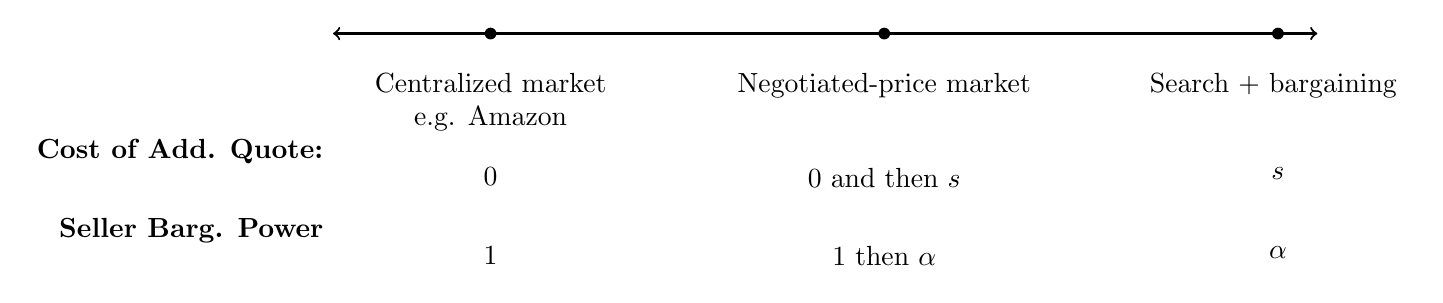
\begin{tikzpicture}[node distance=1cm]
                \draw[<->, thick] (0,0) -- (12.5,0);
                \node (left) at (2,0) [circle, fill=black, inner sep=1.5pt] {};
                \node (mid) at (7,0) [circle, fill=black, inner sep=1.5pt] {};
                \node (right) at (12,0) [circle, fill=black, inner sep=1.5pt] {};
                \node[anchor=east, align=right] at (0, -1.5) {\textbf{Cost of Add. Quote:}};
                \node[anchor=east, align=right] at (0, -2.5) {\textbf{Seller Barg. Power}};
                \node[below=1.5cm of left] {$0$};
                \node[below=1.5cm of mid, align=center] {$0$ and then $s$};
                \node[below=1.5cm of right] {$s$};
                \node[below=2.5cm of left] {$1$};
                \node[below=2.5cm of mid] {1 then $\alpha$};
                \node[below=2.5cm of right] {$\alpha$};
                \node[below=0.3cm of left, align=center] {Centralized market\\ e.g. Amazon};
                \node[below=0.3cm of mid, align=center] {Negotiated-price market};
                \node[below=0.3cm of right, align=center] {Search + bargaining };
            \end{tikzpicture}
        \end{adjustbox}
        %\caption{A continuum of market structures based on seller bargaining power and quoting prices.}
        \label{fig:market_continuum_scaled}
         
    \end{figure}
\note{
Mention that I will not have a feedback slide but will write in red items that I would like to receive feedback on. 

In \textbf{what are aftermarkets} mention that 'search' refers to just the process of costly bargaining. Id DOES NOT necessarily mean that the consumer is learning about a product 

In \textbf{relevance} mention:
\begin{itemize}
    \item Chile there was discussion about the aftermarket and they removed it. 
    \item Aftermarkets are spetially common in platforms. 
\end{itemize}
In \textbf{benchmarks} mention:
\begin{itemize}
    \item One could think about eliminating the first part, do not post prices and only allow for search and bargaining, essentially eliminating the centralized nature of the market or also just allowing firms to post prices.  
    \item In terms of consumer welfare the effects are ambiguous, when comparing the 1st and 3rd case obviously depends on $(s,\alpha)$ and when using the centralized and bargaining stages together then the equilibrium effects are not obvious. 
\end{itemize}
}
   
\end{itemize}
\end{frame}
 
%%%%%%%%%

\begin{frame}
\frametitle{Different use of the aftermarket}\label{slide:single_fig}
\begin{figure}
    \centering
    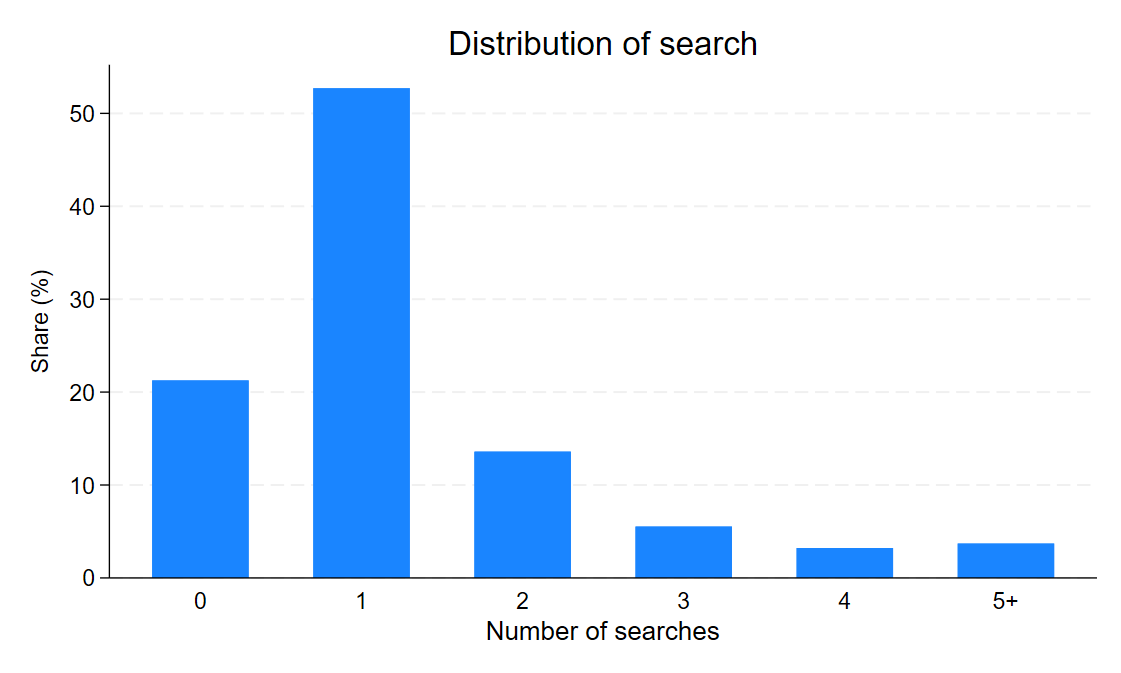
\includegraphics[width=0.49\textwidth]{../figures/IE3_dist_external_offers.png}
    \hfill 
    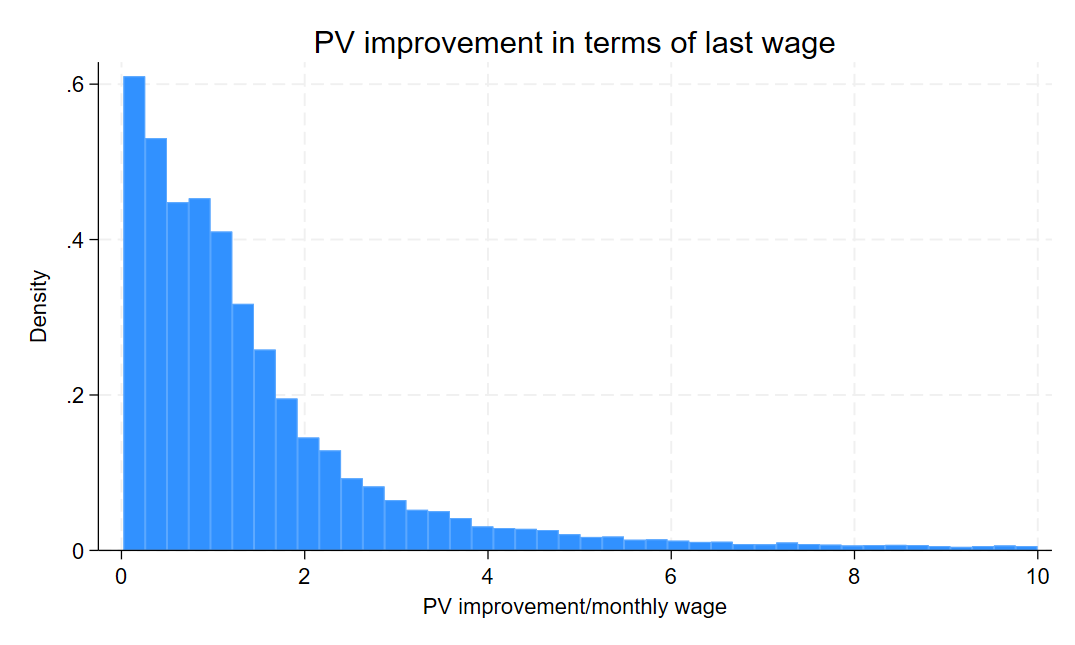
\includegraphics[width=0.49\textwidth]{../figures/IE3_offer_improvement_histogram.png}
\end{figure}

\begin{itemize}
    \item   80\% of the purchases are through the aftermarket 
    \item Poorer households search less \hyperlink{slide:fig4}{\beamerbutton{Evidence}} 
    
    \textcolor{red}{[What are the determinants of search? Search direction?] }
\end{itemize}

\note{That only some people use the aftermarket suggest: 
\begin{itemize}
    \item There are search costs 
    \item Firms could be discriminating based on the search likelihood. 
\end{itemize}
}
\end{frame}

%%%%%%%%%%%%%%%%%%%%%%%%%

\begin{frame}{Literature}
\begin{itemize}
    \item Aftermarkets: \textcite{larsen_efficiency_2021, allen_search_2019}

    \item Competition in selection markets: \textcite{mahoney_imperfect_2017, cuesta_price_2018, cosconati_competing_2025}

    \item Selection in multiple dimensions: \textcite{finkelstein_adverse_2004} and Finkelstein and McGarry (2006).  
\end{itemize}
\end{frame}

%%%%%%%%%%%%%%%%%%%%%%%%%
 
\begin{frame}{Annuities in Chile: SCOMP}  \label{slide:setting}
       
    \begin{itemize}%[<+->]
    \item SCOMP steps: 
    \begin{enumerate}
        \item Request of balance statement 
        \item Request for offers: asks for certain type of contracts (e.g. annuity)
        \item Insurers make offers (e.g. \$1000 per month)
        \item Retiree chooses one of the offers or asks for external offers

    \end{enumerate}

        \item External offers: bargaining and information disclosure
        %When offering insurers know 1. age, 2. amount of savings, 3. gender, 4. dependents. With external offers they learn your RUT(SSN): more information  
    

    \item Firms competition 1. financing cost 2. prediction algorithm 

    \item Profits of firm $j$: 
    \begin{align*}
    \pi_{ji}(F) = S_i-  \mathbb{E}^j_{T} \left[\sum_{t=1}^T\frac{F}{(1+r_j)^t}|x_i \right]
    \end{align*}
    % if it was only financing cost, it would be a monopoly
    \end{itemize}

     $S$: stock of savings, $F$: per period annuity payment, $x_i$: individual mortality factors
    \note{explicitly not link the annuities market with pensions because generates confusion}
\end{frame}

%%%%%%%%%%%%%%%%%%%%%%%%%%%%%%%%%%%%%%

 \begin{frame}{Data} \label{slide:data}
\begin{itemize}
    \item SCOMP data at the individual level  
    \begin{itemize}
        \item Offers received, rejected and accepted 
        \item Total savings 
        \item Demographics: age and gender
    \end{itemize}
     \item Retirement insurance companies: risk ratings, \#  of intermediaries and their  locations.
\end{itemize}
\note{Important to mention that the advantage of our data is that 1) elicits prices from almost all companies and 2) records all the elicited prices. }
\end{frame}

%%%%%%%%%%%%%%%%%%%%%%%
\begin{frame}{Answer the question}\label{slide:answer1}
    \begin{itemize}
        \item Equilibrium model of search and bargaining 
        \begin{itemize}
            \item First stage: sellers bid and consumers buy or search 
            \item Second stage: If buyer searches is matched with a seller and they bargain
        \end{itemize}
        \item Desiderata:
        \begin{itemize}
           \item Imperfect-assymmetric competition\hyperlink{slide:fig2}{\beamerbutton{Evidence}}
            \item Differentiated products   \hyperlink{slide:fig3}{\beamerbutton{Evidence}}
            \item 
        \end{itemize}
    \end{itemize}

    \note{Diff products: if not the case then everyone would choose the highest offer
    
    Imperfect-assymmetric competition: the differences in market share can be due to preferences, but not so the differences in probability of even offering}
\end{frame}


%%%%%%%%%%%%%%%%%%%%%


\begin{frame}{Firm specialization}\label{slide:fig1}    

Firm specialization in groups
\begin{figure}[H]
%\caption{}
\centering{}%
\begin{tabular}{cc}
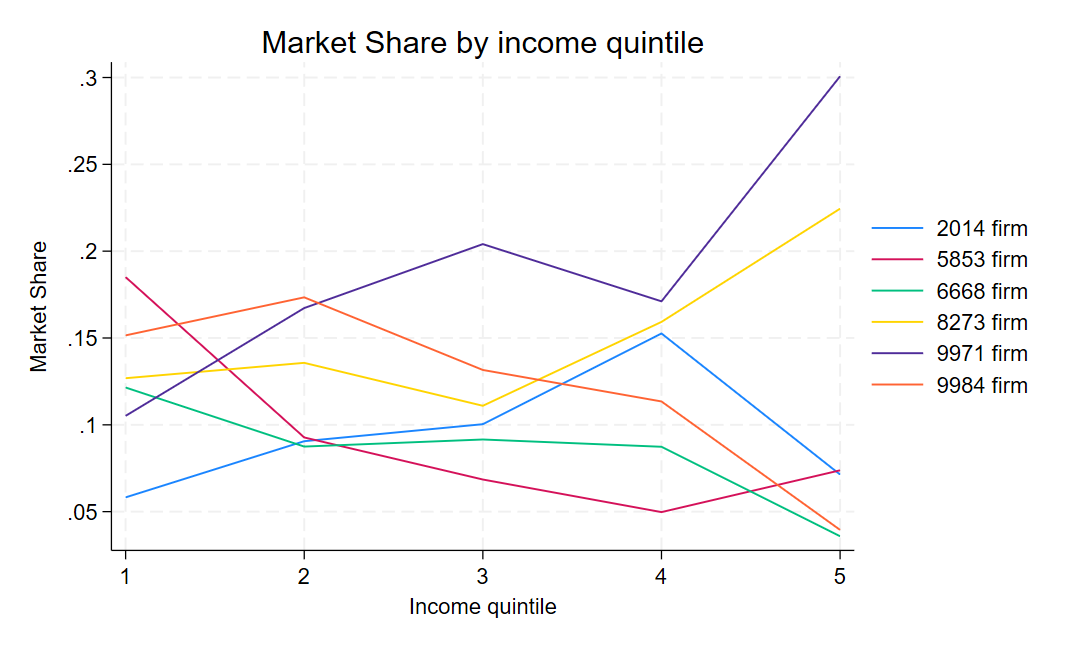
\includegraphics[scale=0.27]{../figures/IE3_supply_income_quintile.png}
\end{tabular}
\end{figure}

\hyperlink{slide:answer1}{\beamerbutton{Go back}}

\end{frame}

%%%%%%%%%%%%%%%%%%%%%

\begin{frame}{Firm specialization(2)}\label{slide:fig2}    

\begin{figure}[H]
\caption{}
\centering{}%
\begin{tabular}{cc}
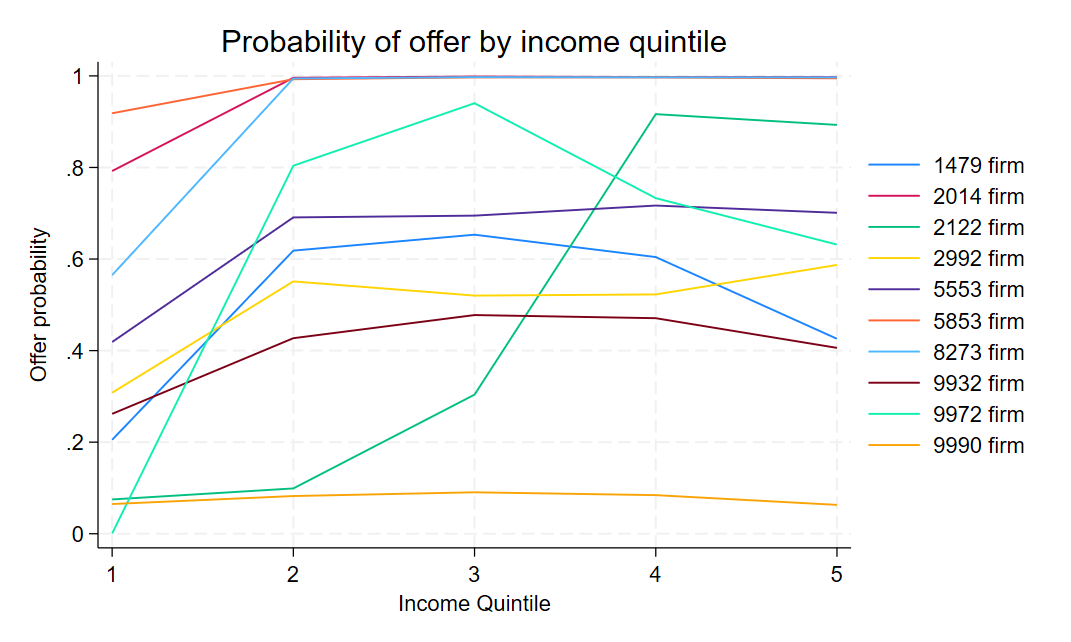
\includegraphics[scale=0.24]{../figures/IE3_supply_offerprob_income_q(2).png}
\end{tabular}
\end{figure}

Firms specialize on buyer types
\hyperlink{slide:answer1}{\beamerbutton{Go back}}

\end{frame}

%%%%%%%%%%%%%%%%%%%%%

\begin{frame}{Heterogeneity in preferences}\label{slide:fig3}    

Buyers do not always buy highest annuity. Average foregone value is 1.57 monthly wages.

\begin{figure}[H]
%\caption{}
\centering{}%
\begin{tabular}{cc}
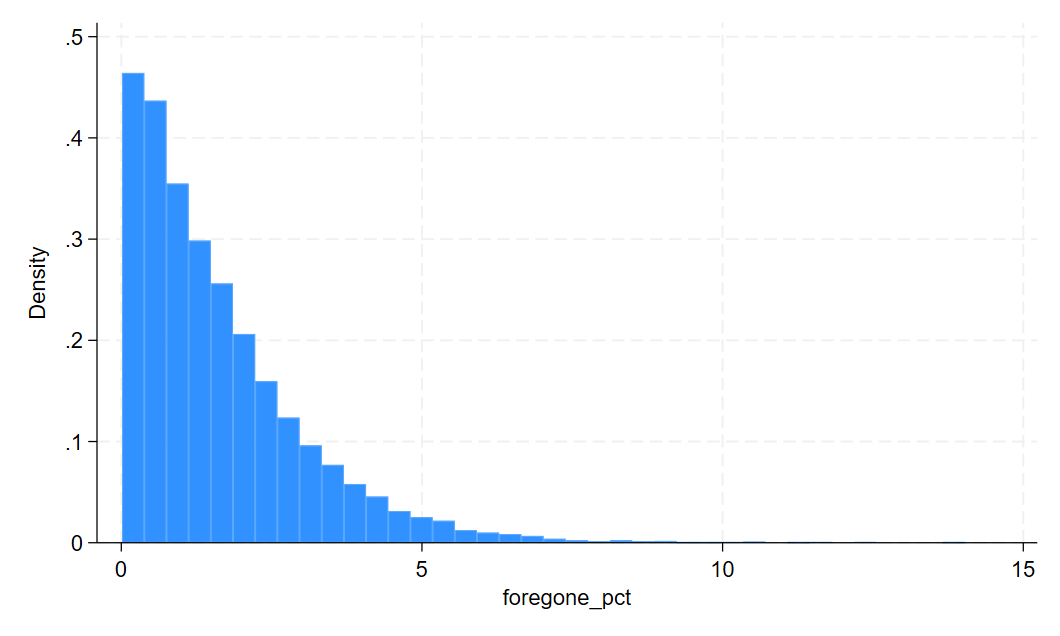
\includegraphics[scale=0.25]{../figures/IE3_foregone_hist.png}
\end{tabular}
\end{figure}
\hyperlink{slide:answer1}{\beamerbutton{Go back}}

\end{frame}

%%%%%%%%%%%%%%%%%%%%%

\begin{frame}{Search(2)}\label{slide:fig4}    

\begin{figure}[H]
%\caption{}
\centering{}%
\begin{tabular}{cc}
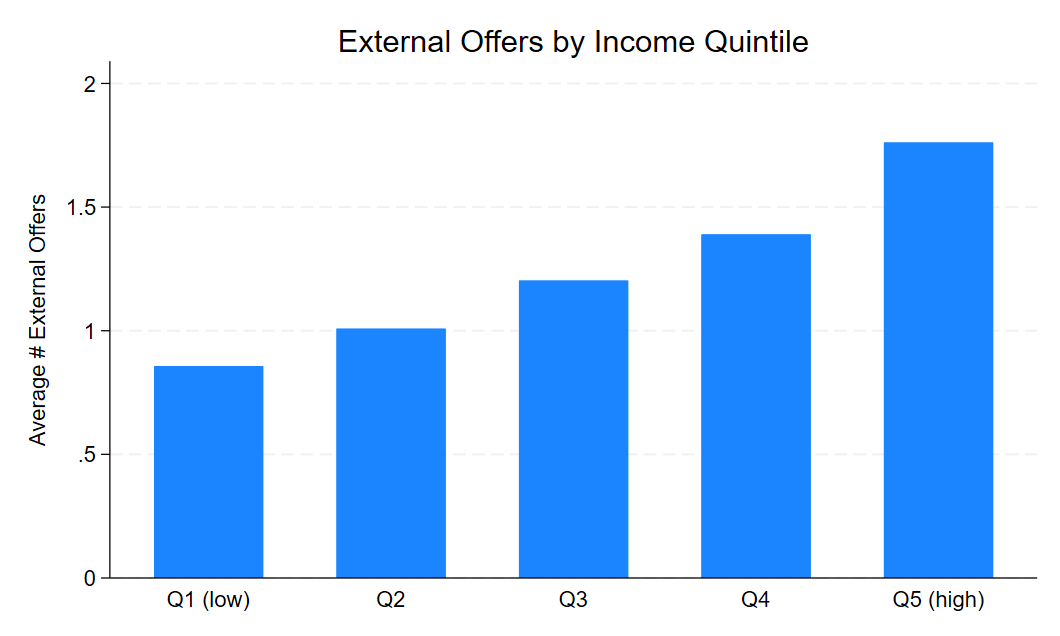
\includegraphics[scale=0.27]{../figures/IE3_search_by_income_quintile.png}
\end{tabular}
\end{figure}
\hyperlink{slide:single_fig}{\beamerbutton{Go back}}
\end{frame}


\end{document}